%------------------------------------------------------------------------------
% Electron diffraction data processing with DIALS
%------------------------------------------------------------------------------
%
%
\documentclass[preprint]{iucr}
%\documentclass[preprint, pdf]{iucr}
  \pdfoptionpdfminorversion=5
  %----------------------------------------------------------------------------
  % Extra packages
  %----------------------------------------------------------------------------
  \usepackage{graphicx}         % For graphics
  \usepackage{mathtools}        % Math stuff
  \usepackage{bm}               % Bold in maths
  \usepackage{listings}         % Code snippets
  \usepackage{bold-extra}       % Bold mono space for code snippets
  \usepackage{url}              % For URLs
  \usepackage{xspace}           % Spacing in macros
  \usepackage{color}            % Colours
  \usepackage{textcomp}         % Required by listings when upquote=true
  \usepackage{gensymb}
	\usepackage{booktabs}
  \usepackage{siunitx}          % Proper formatting for units

  %----------------------------------------------------------------------------
  % Information about the paper
  %----------------------------------------------------------------------------
  \paperprodcode{a000000}
  \paperref{xx9999}
  \papertype{FA}
  \paperlang{english}

  %----------------------------------------------------------------------------
  % Information about journal
  %----------------------------------------------------------------------------
  \journalcode{D}
  \journalyr{2017}
  %\journaliss{1}
  %\journalvol{56}
  %\journalfirstpage{000}
  %\journallastpage{000}
  \journalreceived{\relax}
  \journalaccepted{\relax}
  \journalonline{\relax}

  %----------------------------------------------------------------------------
  % Bits of formatting used throughout document
  %----------------------------------------------------------------------------
  \newcommand{\cctbx}{\emph{cctbx}\xspace}
  \newcommand{\dxtbx}{\emph{dxtbx}\xspace}
  \newcommand{\lstbx}{\emph{lstbx}\xspace}
  \newcommand{\dials}{\emph{DIALS}\xspace}
  \newcommand{\dialsreport}{\emph{dials.report}\xspace}
  \newcommand{\dialsestimategain}{\emph{dials.estimate\_gain}\xspace}
  \newcommand{\dialsfindspots}{\emph{dials.find\_spots}\xspace}
  \newcommand{\dialsindex}{\emph{dials.index}\xspace}
  \newcommand{\dialsrefinebravaislattice}{\emph{dials.refine\_bravais\_lattice}\xspace}
  \newcommand{\dialsrefine}{\emph{dials.refine}\xspace}
  \newcommand{\dialsimageviewer}{\emph{dials.image\_viewer}\xspace}
  \newcommand{\dialsreciprocallatticeviewer}{\emph{dials.reciprocal\_lattice\_viewer}\xspace}
  \newcommand{\ccpfour}{\emph{CCP4}\xspace}
  \newcommand{\labelit}{\emph{LABELIT}\xspace}
  \newcommand{\cctbxxfel}{\emph{cctbx.xfel}\xspace}
  \newcommand{\code}{\texttt}
  \newcommand{\xds}{\emph{XDS}\xspace}
  \newcommand{\mosflm}{\emph{MOSFLM}\xspace}
  \newcommand{\pointless}{\emph{POINTLESS}\xspace}
  \newcommand{\aimless}{\emph{AIMLESS}\xspace}
  \newcommand{\blend}{\emph{BLEND}\xspace}

  % use bold face for vectors
  \renewcommand{\vec}[1]{\mathbf{#1}}
  \newcommand{\mat}[1]{\mathbf{#1}}

  % derivatives
  \newcommand{\pder}[2][]{\frac{\partial#1}{\partial#2}}
  \newcommand{\tder}[2][]{\frac{\mathrm{d}#1}{\mathrm{d}#2}}

  %----------------------------------------------------------------------------
  % Configure the listing environment
  %----------------------------------------------------------------------------

  % Define the Python style
  \definecolor{pykeyword}{rgb}{0,0,0.5}
  \definecolor{pystring}{rgb}{0,0.5,0}
  \definecolor{pycomment}{rgb}{0.6,0.6,0.6}
  \newcommand\pythonstyle{
    \lstset{
      language=Python,
      basicstyle=\scriptsize\ttfamily,
      upquote=true,
      showstringspaces=false,
      otherkeywords={self},
      keywordstyle=\color{pykeyword},
      stringstyle=\color{pystring},
      commentstyle=\color{pycomment},
    }
  }

  % Python environment
  \lstnewenvironment{python}[1][] {
    \pythonstyle
    \lstset{#1}
  } {}

  % use to fix order in bibtex entries
  \newcommand{\mockalph}[1]{}

  % Comments from DW:
  \newcounter{DWCounter}
  \newcommand{\DW}[1]{%
   \stepcounter{DWCounter}%
   {\color{red}{\textbf{DW \#\arabic{DWCounter}: }#1}}%
  }

  % Comments from TG:
  \newcounter{TGCounter}
  \newcommand{\TG}[1]{%
   \stepcounter{TGCounter}%
   {\color{green}{\textbf{TG \#\arabic{TGCounter}: }#1}}%
  }

  % Comments from MC:
  \newcounter{MCCounter}
  \newcommand{\MC}[1]{%
   \stepcounter{MCCounter}%
   {\color{blue}{\textbf{MC \#\arabic{MCCounter}: }#1}}%
  }

\begin{document}

  %----------------------------------------------------------------------------
  % Title of the paper + short title for header
  %----------------------------------------------------------------------------
  \title{Electron diffraction data processing with \dials}
  \shorttitle{\dials for ED}

  %----------------------------------------------------------------------------
  \author[a]{Max T.B.}{Clabbers}
  \author[b]{Tim}{Gruene}
  \author[c]{James M.}{Parkhurst}
  \cauthor[d,e]{David G.}{Waterman}{david.waterman@stfc.ac.uk}{}

  %----------------------------------------------------------------------------
  % Affiliations
  %----------------------------------------------------------------------------

  \aff[a]{Center for Cellular Imaging and NanoAnalytics (C-CINA),
    Biozentrum, University of Basel,
    Mattenstrasse 26,
    4058 Basel, Switzerland}

  \aff[b]{Paul Scherrer Institute,
    5232 Villigen PSI,
    Switzerland}

  \aff[c]{Diamond Light Source Ltd,
    Harwell Science and Innovation Campus,
    Didcot,
    OX11 0DE,
    UK}

  \aff[d]{STFC Rutherford Appleton Laboratory,
    Didcot,
    OX11 0FA,
    UK}

  \aff[e]{CCP4,
    Research Complex at Harwell,
    Rutherford Appleton Laboratory,
    Didcot,
    OX11 0FA,
    UK}

  \shortauthor{Clabbers, Gruene, Parkhurst \& Waterman}

  %----------------------------------------------------------------------------
  % Create the title
  %----------------------------------------------------------------------------
  \maketitle

%------------------------------------------------------------------------------
% Synopsis
%------------------------------------------------------------------------------
\begin{synopsis}

  \DW{synopsis}

\end{synopsis}

%------------------------------------------------------------------------------
% Abstract
%------------------------------------------------------------------------------
\begin{abstract}

  \DW{abstract}
  \MC{added idea for abstract}
  
Electron diffraction is a relatively novel alternative to X-ray crystallography for the 
structure determination of macromolecules from nanometre-sized crystalline sample. 
The short wavelength implies a nearly flat Ewald sphere, affecting the diffraction 
geometry having a low diffraction angle and high sample to detector distance. 
Nevertheless, the DIALS software package can, with specific adaptations, deal with the different geometry 
and successfully proces continuous rotation electron diffraction data. However, pathologies encountered 
specifically in electron diffraction make the data integration more challenging. Uncertainties 
can  arise from instrumentation, e.g. influencing the rotation range per image, or 
lead to distorted diffraction patterns from lens errors.  Dynamic scattering,
Radiation damage, beam drift, uncertainty of rotation axis direction, incomplete wedges 
of data, and strong correlation between lattice parameters and detector distance are a
dditional factors that complicate data integration. Here we show recent features of DIALS 
for electron diffraction, allowing refinement with a varying beam model, applying 
corrections for distorted diffraction images, and enabling joint refinement of multiple 
incomplete wedges of rotation data. These novel features, combined with the existing tools 
in DIALS, make data integration and refinement feasible for electron crystallography, 
even in difficult cases.

\end{abstract}

\newpage

\section{Introduction}

Electron diffraction allows structural analysis of nanometre-sized samples of
crystalline material. Since the maximal radiation dose is proportional to sample
volume, electron diffraction of organic and macromolecular compounds was long
limited to 2D samples\footnote{S. Hovm{\"o}ller, Workshop "Electron
Crystallography of Macromolecular Compounds, 2017}\cite{unwin-henderson:1975}.
In contrast to X--ray crystallography,  the three domains, inorganic, organic,
and macromolecular electron crystallography were developed rather independent of
each other
\cite{vainshtein:1964,dorset:1995,glaeser_downing_derosier:2007,zou:2011}.
Physical and instrumental limitation, like miniature sample size or dynamic
scattering effects and lens distortions, affect \MC{repalce 'lead to much 
worse' with 'affect} data precision.
However, several studies show that model accuracy compares with X--ray
structures \cite{weirich:1996,zeo_adt:2014,dorset:1992,palatinus:2017}. Only
about one and a half decades ago, electron diffraction of 3D crystals was
pioneered with automated diffraction tomography ADT and further refined with
rotation electron diffraction RED
\cite{adt:2007,rotmethod_e:2010,gemmi_adt:2015}. Recently, single crystal 3D electron
diffraction has also been applied for protein crystals
\cite{microed_method:2015,Clabbers2017}. The very recent use of integration
software with profile fitting and scaling is indicative of the independent
development of electron diffraction. These methods have been in use for decades
in X--ray crystallography, improving the quality of diffraction
intensities and their standard uncertainties, whilst enabling heuristic
correction for systematic errors \cite{pflugrath:1999,leslie1999integration}.

\dials is a relatively new package for diffraction integration
\cite{Winter2018}, designed as an extensible toolkit for the implementation of
algorithms relevant to diffraction data analysis. The core set of algorithms
are presented as a suite of command-line programs that can be used following
simple protocols to integrate datasets collected using the rotation method
\cite{Arndt1977}. Many of these algorithms are implementations of tried and
tested methods described in numerous publications over the past three decades
\cite{leslie1999integration,LURE1986phase1and2,LURE1986phase3,kabsch2010xds}.
However, the toolkit design of \dials facilitates the construction of new
algorithms \cite{Gildea2014,Parkhurst2016,Parkhurst2017}. \dials is an
open-source project, allowing scientists from outside the core collaboration to
contribute software, or to use \dials within their own projects \DW{REF
cctbx.xfel, IOTA, any others?}

To date, \dials development has focused on macromolecular and chemical
crystallography datasets, optimised for continuous rotation data collected in
fine slices using photon counting detectors at synchrotron light sources.\MC{maybe this
paragraph could ne omitted?} 
Despite this emphasis, with suitable modification of parameters at certain
steps, high quality results have also been obtained for wide-sliced X-ray
datasets recorded on CCD detectors \cite{dials_adsc:2016a,dials_adsc:2016b}. The common
fundamental assumption is that reciprocal lattice points pass through the Ewald
sphere by constant-velocity rotation around a single axis.
%Reciprocal lattice
%points have a finite extent and the total scattered intensity for one
%reflection is the integration over the reflecting range of slices of
%the reciprocal lattice point that instantaneously satisfy Bragg's law.
No artificial restrictions on the diffraction geometry are imposed, allowing the
modelling of diffraction experiments using a generic vectorial description
\cite{Waterman2016}. By default, two measurements are made for each reflection:
summation integration and three dimensional profile fitting, along with
estimated errors \cite{Winter2018}. The simplicity of this approach, avoiding
assumptions inherent in the details of any particular technique, mean that
\dials is readily adapted for analysis beyond the original scope of its design.

A common feature shared between \dials programs is the global modelling of an
experiment, in which data are assumed to be complete before analysis begins.
This has some advantages over the traditional approach of processing data by
means of a moving window that passes over the complete data set in blocks of a
local range of images. One is that the expensive step of integration can be
performed with a high level of parallelism, as the experimental model is
determined completely ahead of time. A second is that the programs can consider
multiple experiments simultaneously without losing track of the connections
between them. This feature has particular relevance to the global refinement of
diffraction geometry, for which experiments may share some models
\cite{Waterman2016}, certain parameters may be constrained to shift together,
or restraints may be applied between multiple crystal models. These features
can be important for the analysis of electron diffraction datasets, for which
determining accurate diffraction geometry may be challenging
\cite{review_adt_red:2015}, and current
technology usually imposes the collection of incomplete wedges of data for each
crystal. Here we discuss the use of \dials for the analysis of electron diffraction data
that has been collected using the rotation method.

\section{Image formats}

The first stage in processing rotation data with \dials is to import the images
constituting the data set to form a \code{DataBlock}, using the \dxtbx library
\cite{Parkhurst2014}. This library contains format reading classes for the
majority of common file formats used in X-ray crystallography. The classes are
arranged in a hierarchy, from generic classes that contain code to read image
data and construct an experimental model solely from metadata contained in the
image headers, to specific classes that may recognise a particular instrument
and can override for incorrect or missing metadata. This is important for
reading file formats used in electron microscopy because current instruments
usually do not transfer all the information that is required to reconstruct the
experimental geometry. There are three main approaches that can be taken to
import electron diffraction data into \dials.
\begin{enumerate}
  \item Externally convert the native format into a format more common for MX.
  This is the usual approach that has been adopted for data processing with
  other programs such as \mosflm~\cite{leslie2007} and
  \xds~\cite{kabsch2010xds}. For example, data sets have been converted to SMV
  \cite{Hattne2015}, PCK images \cite{Clabbers2017}, or CBF {Gruene2018}.  CBF, the
  Crystallographic Binary Format, \cite{Bernstein2005}, is probably the most
  widely used nowadays. It is a self-describing format combining text strings
  that conform to the imgCIF dictionary to provide comprehensive metadata with
  binary blocks of image data. The reliance on an external conversion tool has
  additional drawbacks.  The possibility of the proliferation of such tools and
  conversion scripts adds complication for the user. As more intermediate steps
  are added the potential for mistakes increases. The fidelity of the conversion
  process must be checked. For example, image export functions within microscope
  vendor-supplied software to common formats such as TIFF might not preserve
  the real pixel intensities, and this fact may not be clear to the user.

  \item Extend the \dxtbx library to recognise native data formats. This
  approach entails writing a format class (typically a single, small Python
  module) to contribute to \dxtbx, following the published description
  \cite{Parkhurst2014} and existing examples. In fact, this may be necessary
  even for data externally converted into a standard MX format. For example, a
  new class derived from a standard MX format base class may be required in
  order to define a mask for certain regions of the images, split a data array
  into multiple panels or ensure appropriate models are created, such as an
  unpolarised beam model. Missing elements of the model can be provided during
  data import by providing parameters at the command line or in a file in the
  PHIL format, a simple data interchange format used within the
  \cctbx~\cite{Grosse-Kunstleve2002}. Appendix~\ref{app:PHIL_example} contains
  an example of such a file. Format classes for native file types that have now
  been added to the dxtbx include image stacks in the TIA Series Data (ESD)
  format used by software provided with FEI microscopes and image stacks in
  Gatan DM4 format.

  \item For local installations, testing or one-off developments for a
  particular data processing problem it may be more appropriate to create a
  format class as a plugin rather than contributing to the \dxtbx library.
  There is no difference in the procedure required to implement the class, the
  resulting Python module should simply be placed in a \code{.dxtbx} directory
  in the user's home area and this will automatically be picked up at runtime
  when required. Various plugins for electron diffraction are collected at
  \url{https://github.com/dials/dxtbx_ED_formats} and can be downloaded and
  modified freely.

\end{enumerate}

\MC{We can add an image of one 1k frame with the correct description and correct geometric positions of each segment as defined in the import plugin for the Timepix cbf’s}

\section{Spot finding \label{sec:spot_finding}}

The spot finding algorithm used in \dials is rather sensitive to the detector
gain. No automatic evaluation of the gain is performed prior to spot finding,
although a value can be determined using the program \dialsestimategain. This
uses the mean and variance of pixels within a region of interest
\cite{leslie2006integration}  and may significantly underestimate the true gain
for detectors that have non-negligible point spread, or corrections applied
that reapportion signal between neighbouring pixels \cite{Waterman2010}.
Experience with CCD detectors shows that setting the gain correctly rather than
estimating it in this manner gives much better spot finding results in \dials,
with far fewer false positives. The format class used to import images must have a
default gain set to an appropriate value, or a suitable value must be passed to
\dialsfindspots for use by the spot finding algorithm. In cases where the
detector gain is not known, the effect on the spot-finding algorithm of setting
different values can be explored interactively using \dialsimageviewer, as shown
in the Figure~\DW{Figure - spotfinding with different gain values. The SMV
TVIPS images are a good example. What is the
right gain for these though?}

\section{Experiment geometry}

The most substantial difference between the processing of rotation data from
electron diffraction compared to X-ray diffraction lies in the modelling of the
diffraction geometry. The short wavelength of an electron beam ($\SI{0.02508}{\angstrom}$
for 200 keV electrons compared to $\SI{1.0332}{\angstrom}$ for 12 keV X-rays) \TG{changed
0.0251 to 0.02508 to match precision} implies a correspondingly large Ewald
sphere, with a small $2\theta$ scattering angle even for the highest resolution
reflections. The low diffraction angles imply a
large effective sample to detector distance to magnify the
diffraction pattern and achieve sufficient spatial separation of peaks. 
Large detectors are advantageous for crystallography
because they allow the sample to detector distance to be increased, which both reduces diffuse
background and improves spatial separation of peaks \cite{Stanton1993}. However, 
in a TEM the detector distance is limited by the largest possible magnification
and the relatively small detectors. Whilst the true detector position underneath the column is
always at a fixed distance, the effective detector distance
is set by the objective lens and does not correspond directly to a quantity that
can be measured mechanically. Similar to an X-ray beamline, the sample to detector distance in
a TEM is easily calibrated with reliable test crystals. However,
inaccuracy in the recorded effective distance may be difficult to correct by the
usual process of diffraction geometry refinement due to the high correlation
between unit cell parameters and the detector distance when
$2\theta_{\text{max}}$ is small, when the Ewald sphere construction becomes
invariant of linear scaling (see Section~\ref{sec:refinement}) \cite{VanGenderen2016}. In addition,
imperfections in the lens system may introduce distortions in the recorded
diffraction images. Possible distortions include
anisotropic magnification where the diffraction pattern pattern is elongated
in one direction, transforming a circular powder pattern to an ellipse \cite{lenscorr_2dx:2006,Clabbers2017}.
Careful alignment of the TEM diffraction setup can reduce these distortions to a minimum.
With disregard of lens defects, the processing software can ignore these
distinctions and model the experiment with an effective detector. The differences between the diffraction
geometry of typical X-ray and electron diffraction cases in real and reciprocal
space are summarised in Figure~\DW{mixed reciprocal-real space Ewald sphere
diagram with detector geometry - like cartoons from the talk? If this can be
done in a way that fits within 2 columns} \TG{the differences are small, but the
consequences are larger - how about a figure that compares the paramters
cross-CC between X-rays and electrons. That has also been part of your talk.}
\DW{I think that is the figure I mean to put in the Diagnostics section}

\MC{rephrased: At an X-ray beamline the sample to detector distance is easily
calibrated with reliable test crystals. Large detectors are advantageous for X-ray crystallography
because they allow the sample to detector distance to be increased, which both reduces diffuse
X-ray background and improves spatial separation of peaks \cite{Stanton1993}.
By contrast, large detector size is a less important factor for electron
diffraction experiments. In that case, the low diffraction angles imply that a
large effective sample to detector distance is required to magnify the
diffraction pattern to fill the detector surface, even for the much smaller area
detectors in use within electron microscopes.  The effective detector distance
is set by the objective lens and does not correspond directly to a quantity that
can be measured mechanically.  With disregard of lens defects
\cite{lenscorr_2dx:2006,Clabbers2017}, the processing software can ignore this
distinction and model the experiment with an effective detector. However,
inaccuracy in the recorded effective distance may be difficult to correct by the
usual process of diffraction geometry refinement due to the high correlation
between unit cell parameters and the detector distance when
$2\theta_{\text{max}}$ is small, when the Ewald sphere construction becomes
invariant of linear scaling (see Section~\ref{sec:refinement}). In addition,
imperfections in the lens system may introduce distortions in the recorded
diffraction images. These may be detected during data processing and under to a
certain extent can be corrected for. The differences between the diffraction
geometry of typical X-ray and electron diffraction cases in real and reciprocal
space are summarised in Figure~\DW{mixed reciprocal-real space Ewald sphere
diagram with detector geometry - like cartoons from the talk? If this can be
done in a way that fits within 2 columns} \TG{the differences are small, but the
consequences are larger - how about a figure that compares the paramters
cross-CC between X-rays and electrons. That has also been part of your talk.}
\DW{I think that is the figure I mean to put in the Diagnostics section}}

Another potential source of inaccuracy in the initial model for the diffraction
geometry arises because of the relatively poor characteristics of the sample
positioning stage of electron microscopes compared to X-ray goniometers for the
purpose of rotation method experiments. Improved set ups are possible
but are not widely available \cite{Yonekura2015,Shi2016}. \DW{more details here?}
\MC{added shi et al 2016, moved the paragraph below to here}
The rotation range per image is generally assumed constant and accurate. This
parameter is not refined by current integration programs. Instruments for used
for electron diffraction should therefore be well calibrated
\cite{gemmi_adt:2015}. Small, smooth deviations from the expected rotation angle
can then be modelled as part of the scan-varying refinement of the crystal.
\TG{Mauro Gemmi pointed me at his calibration method in the cited paper,
therefore I shortened the paragraph}

Generally, there may be
uncertainty regarding the orientation of the rotation axis, the direction of
rotation, and the rotation range per image. A reasonable estimate of the
rotation axis orientation in the plane of the images can be made by finding a
line through the beam centre along which reflections have the widest reflecting
range, and few reflections are found. The direction of rotation around the axis
is more difficult to determine. For an X-ray experiment, the curvature of the
Ewald sphere makes the incorrect choice obvious, for example using a visual
tool such as \dialsreciprocallatticeviewer \cite{Winter2018}. By contrast, the
flatness of the Ewald sphere in electron diffraction ensures that either choice
of handedness of rotation will produce regular reciprocal lattice positions,
as shown by Figure~\ref{fig:invert_axis}. If indexing is successful, it is likely to work
either way. For any case where there is ambiguity, the inverse direction should
also be tested and results compared. The correct solution will have a lower
RMSD for the angular residual between the predicted and observed positions of
the reflections.\TG{I removed my reference to AD3DT and 'uncertainty', and
therefore our both comments.}



\section{Indexing}

Provided a sufficient number of strong spots have been collected (\emph{cf.}
Sec.~\ref{sec:spot_finding}), indexing of electron diffraction works with
similar reliability as with X--ray diffraction data. Difficulties mostly arise
from systematic errors like stability of the rotation axis and, mostly, the
often large variation in oscillation width $\Delta \Phi$.  The \dialsindex
program offers three different methods for determining the unit cell basis
vectors. The default is based on the three-dimensional FFT, but alternatively a
method based on one-dimensional FFT similar to the programs DPS
\cite{Steller1997} and \mosflm \cite{leslie2007} can be used. When the cell
parameters are known, a simplification of the Fourier transform-based methods
can be used that is particularly successful for very narrow wedges of data
\cite{Gildea2014}.  \TG{I removed our comments, this reads good}.

Unless a model space group was chosen by the user, the indexing results are
presented with triclinic symmetry. The compatibility of other choices of
Bravais lattice with the triclinic solution can be tested using the program
\dialsrefinebravaislattice \cite{Winter2018,Sauter2006}. There is no difference
in usage compared with X-ray data, however for electron diffraction data the
results might be more difficult to interpret. In particular, the metric fit
reported for each trial solution \cite{LePage1982} may be large (e.g. greater
than $1^\circ$) even for a correct solution, whereas much smaller values are
expected for good quality X-ray data. The correlation coefficients between
intensities related by symmetry operations of the lattice are affected by data
incompleteness and by factors that cause deviation from expected intensities
such as dynamic diffraction. As a result, these may not be as useful to decide
on the correct lattice as they are in X-ray experiments. The key criterion then
is the RMSD between predictions and observations. A pool of solutions with
RMSDs similar to the original triclinic solution are good candidates. Any
solution resulting in a significant increase in RMSD is suggestive of an
over-constrained lattice and should be discarded.

\section{Refinement \label{sec:refinement}}

\TG{You mention to describe ``protocols''. A typical user would expect a listing
or box that he can enter into Dials w/o too much reading. This section is much
more detailed and better addressed at developers. I would keep the letter but
move the impression of 'protocols' to a different place, like a look-up section
for the impatiend reader.}

Following indexing, the model for the diffraction experiment is refined as
described previously \cite{Waterman2016}. In common with X-ray data processing
with \dials, it is usual to first refine a ``static'' model for the data set,
in which crystal parameters are not allowed to vary across the scan. This
static model is then used as a starting point for scan-varying refinement, in
which the crystal model is allowed to vary in a smooth manner by splitting its
static parameters across the scan and interpolating values using a Gaussian
smoother. The global refinement of a data set improves the stability of the
refinement procedure. However, the geometry of an electron diffraction
experiment raises particular issues that should be taken into account,
especially if data quality is limited by low resolution diffraction for some or
all of the scan, poor quality spot centroids or the scan is an especially
narrow wedge. In this section we offer some practical advice for \dials
refinement tasks with challenging electron diffraction data, when only a single
data set is considered. Section~\ref{sec:group_cell_restraints} presents an
example where the combination of multiple datasets alongside prior
knowledge that the unit cells should be similar is used during refinement as
another way to mitigate difficulties imposed by the diffraction geometry.

The most noticeable problem seen with electron diffraction geometry refinement
is that the accuracy of the refined unit cell may be poor. With $2\theta$ ranges
typical for X--ray data collection, the Ewald sphere construction is gauged by
the radius of the sphere. Deviations from the correct unit cell parameters or
detector distance results in a non--linear deviation of predicted spot positions
across the detector surface. The smaller $2\theta_\text{max}$, the more linear
the deviation becomes and thus more difficult to detect: unit cell volume and
detector distance can be scaled together while maintaining precise spot prediction.
In cases where unit cell imprecision does not prevent structure solution, the
parameters can be refined, as recently implemented in Refmac5 \DW{Note to add a
citation}.  While a change in
the detector parameters can only result in a projective transformation of the
positions of the recorded spots on any image, changes in the cell parameters
will act to move the reciprocal lattice points towards or away from the surface
of the Ewald sphere, altering not only the predicted positions of the spots on
the detector, but also rotation angle and therefore the predicted image number
on which these spots are expected to appear. When the Ewald sphere is
essentially flat, this distinguishing factor is much reduced and it is more
difficult to separate the effects of the detector and unit cell parameters.

The high level of correlation between parameters in diffraction geometry
refinement problems has long been recognised. The method of eigenvalue
filtering was proposed to allow refinement to proceed in such cases
\cite{Reeke1984,LURE1986phase3}, by automatically selecting only those
parameters, or linear combinations of parameters, that have the greatest effect
at each step of refinement. This was deemed necessary to refine crystal
parameters using data from a single oscillation film. Within \dials, we use all
the data available for global refinement, but we usually attempt to refine
simultaneously the beam, crystal and detector parameters. We have seen that
when limited to a narrow wedge of data recorded with the geometry of the
electron diffraction experiment, high correlations are again problematic. \dials
refinement does not use the eigenvalue filtering method, but by default uses a
Levenberg Marquardt algorithm, which provides an alternative approach for
dealing with near-singular least-squares problems. In practice, we find that
this algorithm is robust even in the presence of very high parameter
correlations. However, experience shows that the more challenging problems with
electron diffraction geometry may need many steps before convergence is
achieved, where this is defined as a negligible further reduction in RMSDs. For
this reason, from \dials version 1.8 the maximum number of iterations before
refinement terminates has been raised to 100 from 20 for the Levenberg
Marquardt algorithm. This limit can always be adjusted by the user via the
\code{max\_iterations} parameter.

If a good estimate for the unit cell is available as prior knowledge, this can
be incorporated into refinement by the use of restraints, tying the
unit cell model to an external target. Unit cell restraints are currently
available for static refinement of unit cell models but not scan-varying
refinement, as they were originally developed for XFEL serial crystallography
where scan-varying refinement is irrelevant. The unit cell parameterisation in
DIALS is expressed by using metrical matrix elements as parameters
\cite{Waterman2016}, however for ease of use the restraints are specified in terms of
the real space cell. Each crystal included in refinement can add up to six
restraint terms (for the triclinic case). Irrelevant restraints for cell
parameters that are already constrained by lattice symmetry are automatically excluded. Each
restraint term adds a pseudo-observation to refinement. Taking the cell
parameter $a$ as an example, the pseudo-observation term $R_a$ consists of the squared
residual between that parameter and its target value $a_t$, with a weighting
factor. In common with the real observations, the first derivatives of the
pseudo-observations with respect to the refinable parameters (here, arbitrarily
denoted $p$) are also required for refinement by non-linear least-squares methods.

\begin{equation}
\label{eq:restraint_to_target}
R_a = \frac{\left( a - a_t \right)^2}{\sigma_a^2}
\end{equation}

\begin{equation}
\pder[R_a]{p} = 2 \pder[a]{p} \frac{\left( a - a_t \right)}{\sigma_a^2}
\end{equation}


In principle, statistical weighting could be achieved by
setting the weights equal to the inverse variance of the target cell parameter
values. However, realistic cell parameter uncertainties are notoriously
difficult to obtain \cite{Dauter2015}. For X-ray diffraction refinement we
usually try values between $\sigma \sim 0.001$ for qualitatively ``strong''
restraints and $\sigma \sim 0.1$ for ``weak'' restraints, monitoring the
effect on the refined RMSDs. In the electron diffraction case setting even very
weak restraints to a target cell can avoid issues with the unit cell and
detector distance drifting when these are refined simultaneously. Nevertheless,
the high correlation between these parameters means that the problem of
distinguishing between cell volume and detector distance remains salient, and
indeed the unit cell can be driven towards a target cell of incorrect volume
with minimal increase in refined RMSDs if the detector distance is also
refined. An alternative method of restraining unit cells does not rely on an
external target, but ensures similarity across multiple unit cell models
simultaneously optimised during multi-experiment joint refinement. An example
of this is presented in Section~\ref{sec:group_cell_restraints} and example
\code{PHIL} parameter files for restrained refinement are given in
Appendix~\ref{app:PHIL_example}.

The difficulties with refinement inherent to electron diffraction geometry are
exacerbated during scan-varying refinement of a crystal model, when this is
done jointly with refinement of a static beam and detector model. Like static
refinement, scan-varying refinement in \dials is also global, in that data from
the full rotation scan is used in a single optimisation procedure. However, at
any point in the scan the local values for the crystal unit cell and angular
misset parameters are dominated by the data close to that point. Spot centroids
at rotation angles further from that point have a diminishing effect on the
local crystal model, controlled by a Gaussian smoother. While this allows the
model to express genuine smooth changes to the cell or orientation parameters,
it reduces the stability of the refinement procedure. This has been seen in
cases where a static crystal model allows global refinement of both the
detector and crystal parameters to reasonable values, but scan-varying
refinement of the crystal results in a drift of the average unit cell volume
and detector distance. Despite these observations, scan-varying refinement is
still preferable to static refinement of the beam, crystal and detector models
within local narrow wedges, which suffers even more from high parameter
correlations. To stabilise a problematic scan-varying refinement task we must
either restrain or constrain (fix) some parameters of the model. Currently,
there is no facility available in \dials to restrain the scan-varying unit cell
to the static cell, which is the best (in a least squares sense) overall unit
cell for the dataset. However, such restraints would act to dampen unit cell
variation that may be genuine. A robust alternative approach is already
possible, which is to refine the detector distance only during the static
refinement phase, then fix this parameter during scan-varying refinement. For
particularly recalcitrant cases the detector distance can be fixed for indexing
and again during subsequent refinement jobs so that it remains at the original
nominal value assumed during the import of the data set. This may be
appropriate if the effective distance is well-calibrated. Another option to
improve stability is to modify options for the smoother used in scan-varying
refinement. Each parameterisation of a model that is to be refined in a
scan-varying manner (for example, the crystal unit cell and the crystal
orientation are separate parameterisations) has an associated interval width
parameter that controls the number of refinable subparameters that will be used
to describe changes during the scan. The default interval width is $36^\circ$.
Increasing this value, or directly setting a small absolute number of
intervals, will ensure a greater degree of smoothing.
% because the fall off of
%importance of data far from a point in the scan on the values of parameters at
%that point will be slower.

\section{Diagnostics for problematic diffraction geometry refinement}

\subsection{Simulating data for comparison}

Section~\ref{sec:refinement} describes parameters that need to be adjusted in
difficult cases. To date, even electron diffraction data sets from standard
proteins can be difficult \cite{Clabbers2017,Hattne2015}. At this early
development stage, diagnostic tools are important for fine--tuning parameters.
The program \dialsrefine provides some facilities for
investigating the main issue we have identified, namely the high level of
correlation between the effects of different parameters on the model.
In this section we concentrate on
difficulties arising specifically at very short wavelength typical for  electron
diffraction.  To ensure that the differences we were investigating come as a
result of only the shorter wavelength and greater detector distance, we elected
to compare the results of refinement against simulated data. To generate
simulated spot centroid positions, we started with a real electron diffraction
case consisting of a continuous rotation scan over 35 images with an angular
width of $0.9^\circ$ per image, for a total scan range of $31.5^\circ$. We took
the model for the indexed experiments and ``regularised'' the geometry of the
beam and detector for the purposes of simulation, without changing the crystal
model, which had an orthorhombic unit cell with dimensions $a=\SI{34.17}{\angstrom}$, $b=\SI{73.23}{\angstrom}$
and $c=\SI{110.14}{\angstrom}$. To regularise the beam and detector models, we forced the beam
direction to be exactly aligned to the $-Z$ direction and reoriented the
detector model such that
the beam intersected the detector in the centre of its square window, and the
detector plane was orthogonal to the beam vector. The detector distance
remained at the value of $\SI{1570.98}{\milli\metre}$, which came from the indexing procedure
from the real data set. The original detector model was for a Timepix quad
assembly \cite{VanGenderen2016}, but for simplicity we replaced the four panel
detector model with a single panel model with an equal total extent, thereby
ignoring the gaps between panels. We also removed parallax correction effects
for the regularised model detector, effectively assuming it consists of a
perfectly sensitive plane of zero thickness. The updated electron diffraction
geometry was written to a new \dxtbx experiment list and then altered a second
time to produce regularised geometry for an X-ray experiment. This involved
changing the wavelength from $\SI{0.0251}{\angstrom}$ to $\SI{1.033}{\angstrom}$ and the detector model such
that the total extent and pixel size was equivalent to a Pilatus 6M detector at
a distance of $\SI{200}{\milli\metre}$ from the sample. This model was also written to a \dxtbx
experiment list. The differences between the model geometries are shown in
Table~\DW{Table: diffraction geometry simulation models}.

\DW{Insert Table: diffraction geometry simulation models

Pixel size, distance, wavelength}

\TG{The following (until the end of this section) reads very complicated to me.
As though you describe your learning process: you simulated, faced and overcame
problems, simulated better, with new problems, etc. Maybe you could forget about
your learning process, concentrate on the result and describe only what is
really necessary to understand the underlying model?}
\DW{Yes, I will rewrite this section}

The regularised models were then used alongside the indexed spot list from the
real data set to simulate observed centroid positions for both versions of the
experimental geometry. By using the spot list from a real experiment we ensured
a realistic distribution of strong spots versus resolution. Not all of the
originally found spots can be predicted with the regularised geometry though.
We wanted the differences in refinement runs to be caused only by the
diffraction geometry and not obscured by different sets of input spots.
Therefore, we first found the subset of 2749 reflections from the original spot
list of 2814 reflections that could be predicted by both versions of the
diffraction geometry.
\DW{Perhaps the remainder of this paragraph should be removed. I found it
interesting, but it is perhaps irrelevant: For the electron diffraction geometry, these reflections
covered a total scan range of $33.7^\circ$. Because the indices of strong spots
came from a real electron diffraction experiment, their reciprocal lattice
points lie within a double wedge shaped volume of reciprocal space, bounded by
two planes. The same reciprocal lattice points were also sampled for the
simulation of centroid positions for the X-ray geometry. However, the change of
the Ewald sphere radius means that a much wider total rotation range of
$183.3^\circ$ is required for each of these points to intersect. This is a
direct result of the different sampling volumes implied by the electron
diffraction versus the X-ray diffraction experiment. 90\% of the reciprocal
lattice points intersect the X-ray Ewald sphere within the central $48.9^\circ$
of this range though, with the edges of the scan being much less efficient.
Because the planar wedge of reciprocal lattice points is excited very unevenly
during the simulated X-ray scan we should not use this method to simulate data
for a test of scan-varying refinement. However, for global static refinement of
beam, crystal and detector parameters, the rotation angle of each spot is not
important; rather it is the difference between that and the predicted angle
that is relevant. Although the spot list going into refinement for the X-ray
geometry simulation was not realistic for an X-ray scan, using the same spots
for both the X-ray and electron diffraction simulations was a simple way to
ensure that the differences we see in refinement behaviour were due only to the
modelling of the diffraction geometry.}

Simulated centroid positions were calculated for each version of the geometry
by predicting their positions then adding random error. The random errors were
drawn from a normal distribution with a standard deviation of 0.25 pixels for
the $X$ and $Y$ positions and 0.25 images for the $Z$ position. For real data,
the centroid position errors in $X$, $Y$ and $Z$ are neither independent, nor
normally-distributed. However, the purpose of adding displacements to the
centroid positions was merely to ensure than refinement would proceed to
convergence with realistic final RMSDs. The centroid positions from
spot-finding result from a centre-of-gravity calculation, which also provides
estimated errors in these positions that are used to set weights in
refinement. These errors have a dependence on the found spot intensity. Rather
than simulating new error estimates, for simplicity we kept the original error
estimates from spot-finding on the real data set to give a realistic
distribution of weights. The centroid $X$, $Y$ positions and their errors were
rescaled to units of millimetres for use in refinement using the pixel sizes
shown in Table~\DW{ref Table above: diffraction geometry simulation models}.

\subsection{Refinement diagnostics}

\DW{Introduce this section differently. Both types of diagnostic are based on
the Jacobian matrix. Introduce that briefly first, then describe the
complementary information from the qualitative corrgrams and the
condition number, without implying that the development of the second diagnostic
was a response to deficiencies in the first.}

Refinement was performed for both versions of the geometry, using default
settings in \dialsrefine. In each case, 13 parameters were refined in total:
six to describe the detector position and orientation, one beam orientation
angle, three crystal orientation angles and three metrical matrix parameters
for the unit cell. Graphical ``corrgrams'' were created for the final step of
refinement in each case. These diagrams are a way of rapidly assessing
correlations between the parameters of refinement in a visual manner. Since
their introduction, described in \citeasnoun{Waterman2016}, this diagnostic has
been improved. Rather than combining data in a single corrgram, the three
dimensional nature of the centroid data is respected and three corrgrams are
produced: one for each of the dimensions $X$, $Y$ and $\phi$. These separate
figures are more appropriate for assessing the levels of correlations between
parameters implied by the data, whereas a single corrgram can obscure these
features because the derivatives of calculated centroid positions with respect
to some parameter $\pder[X]{p}$, $\pder[Y]{p}$ and $\pder[\phi]{p}$ come from
different distributions and thus should not be combined in a meaningful
calculation of correlation.

The two sets of three corrgrams are shown in the supplementary figure
\DW{reference to this}. The pattern of high correlations between parameters
that affect the predicted reflection positions $(X, Y)$ on the detector
plane are similar in the cases of electron and X-ray diffraction
geometries. However, in general, the absolute values of correlations are higher
for the electron diffraction geometry. The most striking difference between the
two cases is shown on the corrgram for the parameters that affect the predicted
rotation angle, $\phi_c$. None of the detector parameters affect $\phi_c$, so
only the beam and crystal parameters are of interest. The relevant subset of
the corrgram is reproduced in Figure~\DW{see below}, which shows that absolute
correlations between all parameters in this block are high for the electron
diffraction geometry.

The inspection of corrgrams may provide a qualitative indication of parameters
that may cause problems during geometry refinement, but it can be difficult to
interpret the details of these plots. Seeing as certain correlations are high
anyway even in unproblematic cases, it is also not easy to determine simply
from these plots which cases actually will be troublesome. For these reasons,
we investigated an alternative diagnostic with a simpler interpretation. Each
step of a non-linear least squares problem is expressed as a linearised
sub-problem of the form

\begin{equation}
  \label{eq:linearised_step}
  \mat{J} \vec{\Delta p} = \vec{\Delta r}.
\end{equation}

By convention, the three-dimensional observations are split so that
$\vec{\Delta r}$, the vector of residuals, contains first the $(X - X_o)$
components, followed by the $(Y - Y_o)$ components, and finally the $(\phi -
\phi_o)$ values. $\mat{J}$, the Jacobian matrix of first partial derivatives of
the residuals with respect to each parameter of the problem, is thus similarly
formed in blocks, with the upper third of the matrix corresponding to
$\pder[X]{p}$ values, the second to $\pder[Y]{p}$ and the lower third to
$\pder[\phi]{p}$. The vector $\vec{\Delta p}$ is the parameter shift vector to
be determined for the step. The corrgram diagnostic investigates correlation
between columns within each block of the Jacobian, identifying which parameters
are the least distinguishable from each other, but might not give a clear
indication of which refinement cases will actually cause problems. By contrast,
calculating the condition number of $\mat{J}$ provides a measure of how
well-posed is the sub-problem given by Equation~\ref{eq:linearised_step}, but
does not pick out which parameters are culpable. A condition number $\kappa
\left( \mat{J} \right)$ of infinity means that $\mat{J}$ is singular, while a
finite value of $\kappa \left( \mat{J} \right)$ gives a bound on the accuracy
of the solution to Equation~\ref{eq:linearised_step}. We added an optional
diagnostic to \dialsrefine to calculate $\kappa \left( \mat{J} \right)$ for
each step of refinement, and used this during the refinement of the two cases
presented here. For the final step of refinement prior to termination at RMSD
convergence the condition number for the electron diffraction geometry $\kappa
\left( \mat{J}_{\textrm{ED}} \right) \approx 5 \times 10^5$ while for the X-ray
diffraction geometry $\kappa \left( \mat{J}_{\textrm{MX}} \right) \approx 2
\times 10^3$. This clearly indicates that the electron diffraction geometry
presents a considerably less well-posed problem for refinement.

The Jacobian used to calculate both the corrgram and the condition number
diagnostics does not include blocks related to pseudo-observations that may be
used as restraints in refinement. For that reason, it should be noted that the
diagnostics give information about underlying degeneracy of parameters
determined only by the geometry of the problem, not including the effects of
modifications to the problem that may have been introduced to improve the
robustness of the procedure. Similarly, the diagnostics inform us directly
about properties of the normal equations of the Gauss-Newton problem implied by
Equation~\ref{eq:linearised_step} rather than the modified normal equations of
the default Levenberg-Marquardt algorithm that is typically in fact used to
find the solution. This ensures that these diagnostics can be used to warn us
of problems with the set up of the diffraction geometry refinement itself,
without conflation with factors relating to implementation details of the
algorithm used to perform the optimisation.

\section{Multiple crystal restrained refinement \label{sec:group_cell_restraints}}

A powerful feature of \dials is multiple experiment joint refinement, whereby
models that can be shared between data sets are refined simultaneously with
models that differ between data sets. A typical use case for X-ray
crystallography would be for multiple data sets of crystals that were collected
without changes to the beam, goniometer and detector between data collection
runs. In such a case, the beam, goniometer and detector models can be refined
against the combined data from all of the runs, whilst the crystal models are
simultaneously refined against the data specific to each run. This reduces
correlation between the parameters of the shared and individual models,
improving the parameter estimates for every model \cite{Waterman2016}. As
electron diffraction data sets are often individually incomplete due to the
restricted tilt range of commonly used sample stages, many of the protein
structures reported to date have been refined against data merged from multiple
crystals \cite{Yonekura2015,Clabbers2017,DelaCruz2017}. It would seem therefore
that multi-experiment joint refinement has a place in electron crystallography,
too.

Electron crystallography takes place at nanometre scale. The required precision
is available, but has so far not been assembled for electron microscope
\cite{nm_gonio:2013,prigo:2015} instruments, and electron microscopes are not
dedicated for diffraction.  Generally, it is safer to assume that truly
reproducible experimental geometry cannot be achieved between runs, and models
cannot be shared. Even so, it is still possible to benefit from joint
refinement by providing other links across
experiments. \dials allows two approaches to this.

\begin{enumerate}
  \item Constraints, in which equivalent parameters (such as the detector
  distance) are linked between separate models such that their values will
  shift by equal amounts at each step of refinement. This has not been explored
  yet in the context of electron diffraction and will not be discussed further.
  \item Unit cell restraints, in which equivalent cell parameter values across
  multiple crystals are linked by a similarity restraint.
\end{enumerate}

%The difficulties in refining accurate unit cell parameters for electron
%diffraction experiments may cause uncertainty when it comes to choosing
%datasets for joint scaling and merging. Indeed, the program \blend
%\cite{Foadi2013} relies on cell parameters to perform hierarchical cluster
%analysis that can be used to identify probable outliers. For
%individually-refined electron diffraction datasets, differences in the cells
%due to problematic refinement is likely to mask true differences due to
%non-isomorphism.


Electron diffraction experiments yield very large uncertainties for the unit
cell parameters. By jointly refining multiple data sets with a restraint that
ties the individual cell parameters to their mean values, the overall variation
in the cell parameter values will be reduced. The strength of each restraint can
be adjusted by setting $\sigma$ values, as described before in
Section~\ref{sec:refinement}. These can be optimised to find the point that
minimises the variation in cell parameter values whilst retaining acceptable
refined RMSDs \DW{Figure: choosing restraint strength}. Setting $\sigma$
values below that point would decrease the variation in the cells further, but
at a cost of poor RMSD, indicating that such a small variation in cell
parameters is not compatible with the data.

\TG{Question: does DIALS recommend integration in P1? XDS does so, but I don't
think many protein crystallographers do that, me included. For ED this may
improve data quality, and this would greatly support your point, because with
P1, one still has to find the appropriate cell. Worth trying?}
\DW{No, we don't usually recommend integrating in P1.
In the very few cases I tried (MX data) constraining the cell symmetry
tended to make slight improvements to integrated data quality. In the presence
of systematic errors in the experiment geometry though, I can imagine how relaxing
the lattice constraint may result in better data quality by ``mopping up'' some
of these errors. When I find a good example for this section (288 not looking
like the best candidate now) I will try both with and without lattice constraints}

\DW{Figure: choosing restraint strength - plot sigma versus average RMSD
for multiple refinement trials to pick a suitable restraint strength}

No external target cell is required, so this method is suitable for new
projects without prior knowledge of cell parameters. Because the mean values
change as the cell parameters are refined, there is essentially a moving target
that changes at each step of refinement. In principle then, this method is
unable to break the ambiguity between individual cell volumes and their
associated detector distances. However, in practice the combination of multiple
datasets seems to help avoid these correlated features drifting to clearly
erroneous values, possibly by resampling systematic errors that may drive such
drifts in individual cases, or by determining the cell parameters against data
with overall greater completeness.

In common with restraints to target shown by
Equation~\ref{eq:restraint_to_target}, each crystal $i$ can add up to six
restraints terms, expressed as pseudo-observations of the form

\begin{equation}
R_{a_i} = \frac{\left( a_i - \langle a \rangle \right)^2}{\sigma_a^2}.
\end{equation}

The derivative of this pseudo-observation with respect to the parameters of crystal $i$ is

\begin{equation}
\pder[R_{a_i}]{p_i} = 2 \pder[a_i]{p_i} \left( 1 - \tfrac{1}{n} \right) \frac{\left( a_i - \langle a \rangle \right)}{\sigma_a^2}.
\end{equation}

Because the mean changes at each step, the derivative of the
pseudo-observations of each other crystal $j$ with respect to the parameters of
crystal $i$ must also be calculated

\begin{equation}
\label{eq:cross-crystal-deriv}
\pder[R_{a_j}]{p_i} = -\frac{2}{n} \pder[a_i]{p_i} \frac{\left( a_j - \langle a \rangle \right)}{\sigma_a^2}.
\end{equation}

This fact means that the restraints block of the Jacobian matrix used in
refinement is a dense matrix. This has performance implications for joint
refinement where group restraints are applied over large numbers of crystals,
for example with XFEL data sets. In such cases, an option is provided to ignore
the cross-crystal gradient terms of Equation~\ref{eq:cross-crystal-deriv}. For
most cases with electron diffraction data sets, joint refinement with a few
tens of crystals is tractable without this approximation.

To demonstrate the use of unit cell similarity restraints with electron
diffraction data, \DW{Finish section based on Max's lysozyme data}
%we processed 10 publicly-available datasets from crystals of
%Trypsin \cite{sbdb288}, downloaded from
%\url{http://dx.doi.org/10.15785/SBGRID/288} and converted to SMV format
%following the instructions provided, including a correction for low pixel
%counts that are truncated to zero \cite{Hattne2016}.

\section{Discussion}
\DW{discussion and conclusions here.}

%------------------------------------------------------------------------------
% Acknowledgements
%------------------------------------------------------------------------------
\ack{Acknowledgements

  \DW{acknowledgements}

}

%------------------------------------------------------------------------------
% References
%------------------------------------------------------------------------------
\referencelist[DIALS_for_ED]

     %-------------------------------------------------------------------------
     % TABLES AND FIGURES SHOULD BE INSERTED AFTER THE MAIN BODY OF THE TEXT
     %-------------------------------------------------------------------------

     % Simple tables should use the tabular environment according to this
     % model

\begin{figure}
  \label{fig:invert_axis}
  \centering
  \caption{
    Five reciprocal lattice points are shown (in black and labelled) along the
    $a^*$ axis for a crystal with unit cell dimension $a=\SI{10}{\angstrom}$.
    Arcs representing the surface of the Ewald sphere with a typical X-ray
    wavelength of $\lambda=\SI{1.0332}{\angstrom}$ intersect these points at
    rotation angles between $15.0^\circ$ for $h=1$ to $27.0^\circ$ for $h=5$,
    where rotations are assumed to be clockwise from vertical in the plane of
    the figure. If the modelled rotation axis is inverted then $\phi$-centroids
    of observed spots would be mapped onto Ewald spheres rotated between
    $-15.0^\circ$ and $-27.0^\circ$, resulting in a distinct curvature to the
    reconstructed reciprocal lattice (points shown in blue). In the case of
    electron diffraction at $\lambda=\SI{0.02508}{\angstrom}$ the spots are
    almost observed simultaneously, at rotation angles between $12.1^\circ$ and
    $12.4^\circ$. For clarity a single Ewald arc is shown, for $h=3$. If the
    assumed axis is inverted then $\phi$-centroids between $-12.1^\circ$ and
    $-12.4^\circ$ still result in almost a straight line (points shown in
    green). It is therefore difficult to determine the correct direction of
    rotation from the appearance of the reconstructed reciprocal lattice alone.
  }
  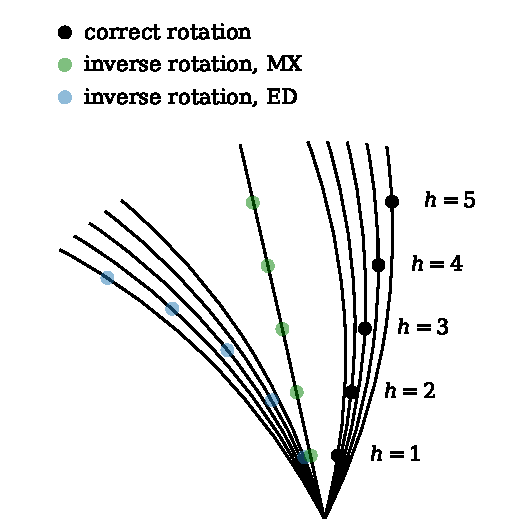
\includegraphics[width=0.5\textwidth]{Figures/relps_inverted_axis.pdf}
\end{figure}

\appendix

\section{\code{PHIL} examples \label{app:PHIL_example}}

\DW{PHIL example for overriding geometry on import}

\DW{PHIL example for setting unit cell restraints}

\end{document}
